
\documentclass[ms.tex]{subfiles}
\begin{document}

\section{Galactic Properties}
\label{sec:galprops}

% fig 1
\begin{figure*}
\centering
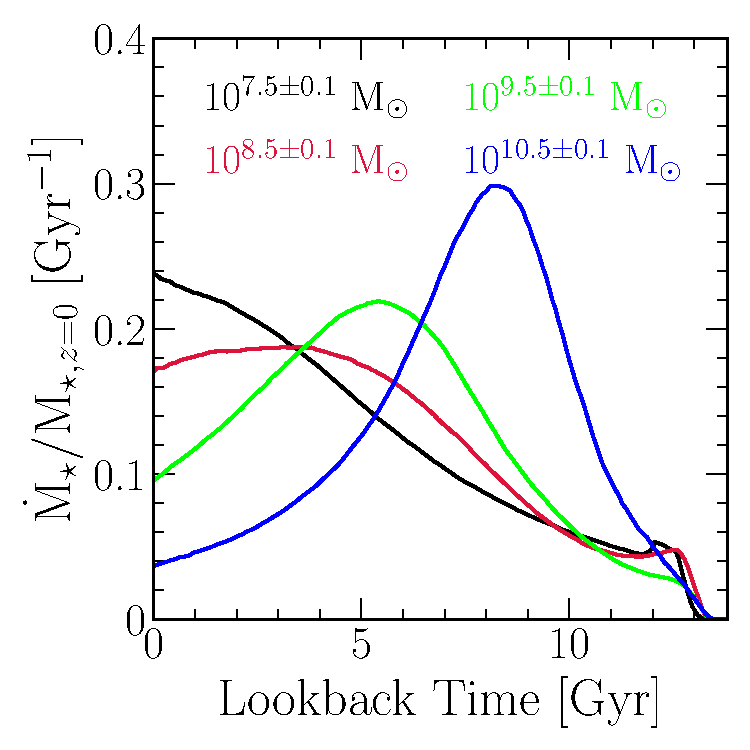
\includegraphics[scale = 0.43]{umachine_sfhs.pdf}
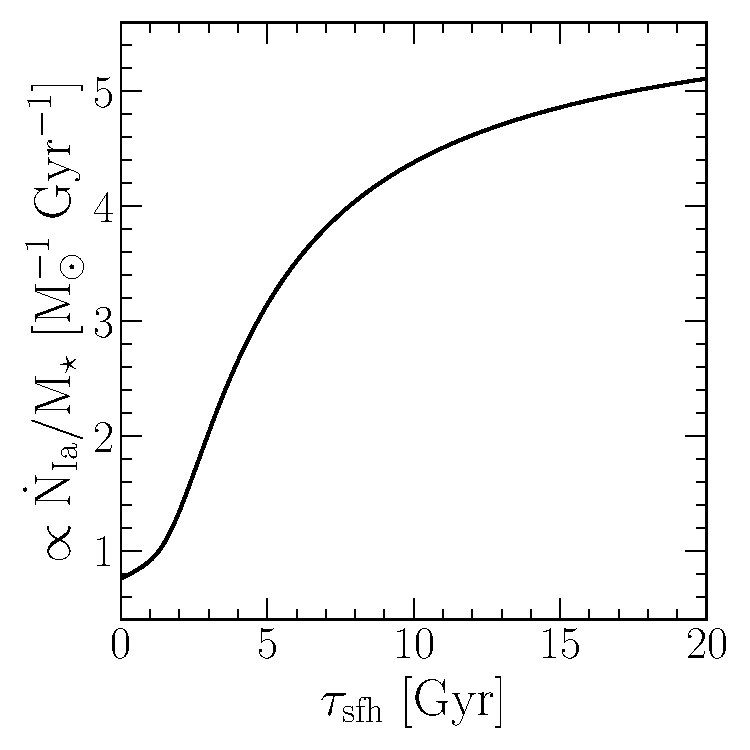
\includegraphics[scale = 0.42]{iarate_vs_tausfh.pdf}
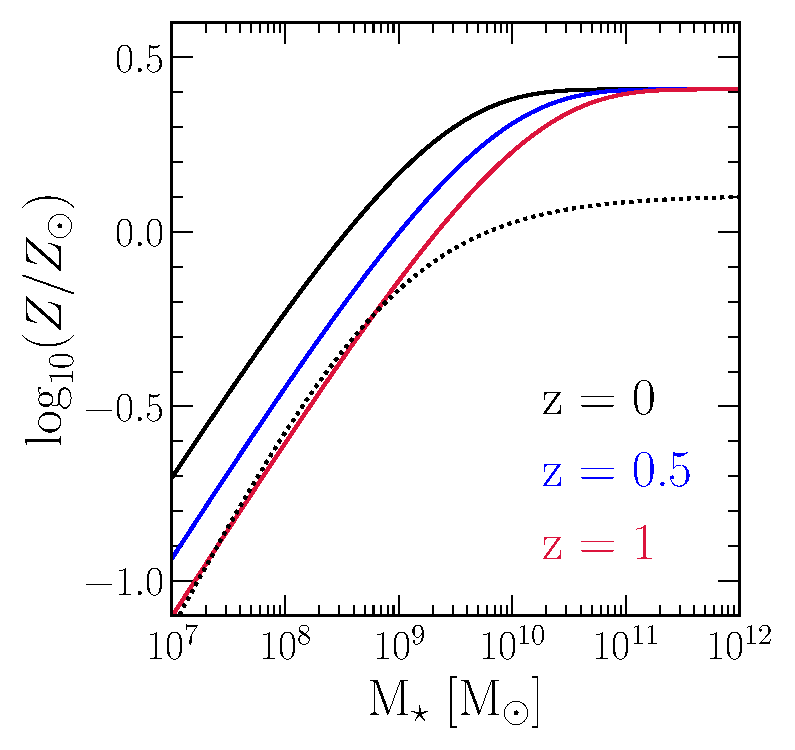
\includegraphics[scale = 0.42]{mzr.pdf}
\caption{
\textbf{Left}: The best-fit mean SFHs of the~\um~galaxies with present-day
stellar masses of $\mstar = 10^{7.5 \pm 0.1}$ (black),~$10^{8.5 \pm 0.1}$ (red),
$10^{9.5 \pm 0.1}$ (green), and $10^{10.5 \pm 0.1} \msun$ (blue) normalized by
their present-day stellar masses.
\textbf{Middle}: The specific SN Ia rate as a function of the e-folding
timescale of the SFH~$\tau_\text{sfh}$ assuming a linear-exponential time
dependence and a~$\tau^{-1}$ power-law SN Ia DTD.
\textbf{Right}: The redshift-dependent MZR reported by~\citet{Zahid2014} at
$z = 0$ (black solid),~$z = 0.5$ (blue), and~$z = 1$ (red).
For comparison, we include the~$z \approx 0$ MZR measured by
\citet[][black dotted]{Andrews2013}.
}
\label{fig:sfh_mzr}
\end{figure*}

We begin by examining how the mean galactic SFH varies with present-day stellar
mass as predicted by the~\um~semi-analytic model~\citep{Behroozi2019}.
Using dark matter halo properties supplied by the~\textit{Bolshoi-Planck} and
\textit{Multi-Dark Planck 2} dark matter only simulations~\citep{Klypin2016,
RodriguezPuebla2016},~\um~follows a conventional semi-analytic model framework
(see, e.g., the review in~\citealt{Somerville2015a}) and successfully
reproduces a broad range of well-constrained observables, including stellar
mass functions, cosmic SFRs, specific SFRs, quenched fractions, and UV
luminosity functions.
While some semi-analytic models have used the extended Press-Schechter
formalism~\citep{Press1974, Bond1991} to generate halo merger trees and push
the lower stellar mass limit of their model down to~$\mstar \approx 10^7~\msun$
\citep[e.g.][]{Somerville2015b}, an advantage of~\um~is that the high mass
resolution of~\textit{Bolshoi-Planck} and~\textit{Multi-Dark Planck 2}
allows merger trees down to~$\mstar = 10^{7.2}~\msun$ to be obtained directly
from the simulations.
Conveniently, this limit is approximately the lowest mass for which there are
empirical constraints on the specific SN Ia rate from ASAS-SN~\citep{Brown2019}
and DES~\citep{Wiseman2021}.
In the interest of relating these predictions to data from ASAS-SN
\citep{Shappee2014, Kochanek2017}, an untargeted survey, we take the full
galaxy sample from~\um, including both star forming and quenched galaxies as
well as both centrals and satellites, though centrals are the dominant
population across the full stellar mass range.
\par
In the left panel of Fig.~\ref{fig:sfh_mzr}, we plot the best-fit mean SFH as a
function of lookback time in four narrow bins of observed stellar mass taken
from~\um.
In general, low stellar mass galaxies have more extended SFHs than their
higher mass counterparts.
This effect is sufficiently strong that for stellar masses of
$\sim$$10^{7.5}~\msun$, typical SFRs are still increasing at the present day
while~$\sim$$10^{10.5}~\msun$ galaxies experienced their fastest star formation
long ago.
\par
We adopt a DTD that scales with the age of a stellar population as~$\tau^{-1}$
as suggested by comparisons of the cosmic SFH with the volumetric SN Ia rate
as a function of redshift (\citealp{Maoz2012a};~\citealp*{Maoz2012b};
\citealp{Graur2013, Graur2014}).
We have reconducted our analysis using alternative choices of the power-law
index as well as an exponential DTD with an e-folding timescale of
$\tau_\text{Ia} = 1.5$ Gyr and found similar conclusions in all cases.
In principle, the minimum delay of the DTD could be as short as~$\sim$40 Myr if
WDs are produced by~$\lesssim$8~\msun~stars~\citep*[e.g.,][]{Hurley2000}, and
perhaps even shorter at low metallicity if the total metal content of a star
significantly impacts its lifetime as in, e.g.,~\citet{Kodama1997} and
\citet{Vincenzo2016}.
However, if SNe Ia require some additional time following WD formation, the
minimum delay will be longer.
Since we are interested in the first-order effects of variations in the SFH on
specific SN Ia rates, we assume a value of~$t_\text{D} = 100$ Myr.
We have also reproduced our calculations with both~$t_\text{D} = 40$ Myr and
$t_\text{D} = 150$ Myr and found similar results in both cases.
\par
% \par
% Although the details of the SN Ia DTD have been a topic of active inquiry for
% some time~\citep[e.g.][]{Greggio2005, Strolger2020, Freundlich2021},
% comparisons of the cosmic SFH~\citep[e.g.][]{Hopkins2006, Davies2016, Madau2014,
% Madau2017, Driver2018} with the volumetric SN Ia rate as a function of redshift
% suggest that the cosmic DTD is broadly consistent with a~$\tau^{-1}$ power-law
% (\citealp{Maoz2012a};~\citealp*{Maoz2012b};~\citealp{Graur2013, Graur2014}).
% A DTD of approximately this form is also expected under the double-degenerate
% scenario given population synthesis models of binary white dwarfs and the loss
% of angular momentum due to graviational wave emission (e.g.
% \citealp{Mennekens2010};~\citealp*{Maoz2014}).
% We therefore adopt this parametrization in this paper, though we have
% reconducted our analysis using an exponential DTD with a timescale of
% $\tau_\text{Ia} = 1.5$ Gyr and found similar results.
% We do not consider metallicity-dependent variations in the shape of the DTD
% here, instead focusing on the overall normalization.
% \par
% In principle, the minimum delay time of the DTD could be as short as~$\sim$40
% Myr if WDs are produced by~$\lesssim 8~\msun$ stars~\citep*[e.g.][]{Hurley2000},
% and perhaps even shorter at low metallicity if the total metal content of a
% star significantly impacts its lifetime as in, e.g.,~\citet{Kodama1997} and
% \citet{Vincenzo2016}.
% However, if SNe Ia require some additional time following WD formation, the
% minimum delay will be longer.
% Since we are interested in demonstratin the first-order effects of variations
% in SFHs on specific SN Ia rates, we assume a value of~$t_\text{D} = 100$ Myr.
% We have also reproduced the results of this paper with both~$t_\text{D} = 40$
% Myr and~$t_\text{D} = 150$ Myr and found similar results in both cases.
% \par
For an SFH~$\dot{M}_\star$ and DTD~$R_\text{Ia}$ as functions of lookback time
$\tau$, the specific SN Ia rate at a stellar mass~$\mstar$ is
\begin{equation}
\frac{\dot{N}_\text{Ia}(M_\star | \gamma)}{M_\star} \propto Z(M_\star)^\gamma
\ddfrac{
	\int_0^{T - t_\text{D}}\dot{M}_\star(\tau | M_\star) R_\text{Ia}(\tau) d\tau
}{
	\int_0^T \dot{M}_\star(\tau | M_\star) d\tau
}
\label{eq:specia}
\end{equation}
where~$T = 13.2$ Gyr is the time elapsed between the onset of star formation
and the present day.
To investigate the effects of metallicity, we add a power-law
$Z(\mstar)^\gamma$ where~$Z$ is given by the MZR.
We are only interested in the scaling of the rates with~\mstar, so we normalize
all rates to unity at~$\mstar = 10^{10}~\msun$ following~\citet{Brown2019}.
Although the denominator of equation~\refp{eq:specia} in detail should depend
on mass loss from stars as they eject their envelopes, this is an approximately
constant term which can safely be neglected in the interest of computing
relative rates ($\approx$40\% for a~\citealt{Kroupa2001} IMF; see discussion
in~\S\S~2.2 and 3.7 of~\citealt*{Weinberg2017}).
\par
To qualitatively illustrate how the specific SN Ia rate scales with how prompt
or extended the SFH is, we consider the simple example of a linear-exponential
parametrization~$\dot{M}_\star \propto te^{-t/\tau_\text{sfh}}$ where
$t = T - \tau$.
The middle panel of Fig.~\ref{fig:sfh_mzr} shows equation~\refp{eq:specia} as
a function of the e-folding timescale~$\tau_\text{sfh}$ assuming~$\gamma = 0$.
The specific SN Ia rate is slowest in the limiting case of a single episode of
star formation (i.e.~$\tau_\text{sfh} = 0$), rises steeply until
$\tau_\text{sfh} \approx 10$ Gyr, and then flattens once
$\tau_\text{sfh} \gtrsim T$.
A higher specific SN Ia rate as observed in dwarf galaxies is therefore a
natural consequence of their more extended SFHs, though we demonstrate below
that this effect accounts for only a factor of~$\sim$2 between~$10^{7.2}$ and
$10^{10} \msun$.
% \par
% Not only do dwarf galaxies have more extended SFHs, but the empirical MZR
% indicates that they also have a lower metal content~\citep{Tremonti2004,
% Gallazzi2005, Zahid2011, Kirby2013}.
% At low metallicities, there are multiple effects which could increase the SN Ia
% rate.
% At fixed initial mass, low metallicity stars leave behind more massive WDs due
% to weaker winds and consequently enhanced core growth during the AGB phase
% \citep{Umeda1999, Willson2000, Marigo2007, Meng2008, Zhao2012, Kalirai2014}.
% This effect could make it easier for a WD to reach the Chandrasekhar mass and
% explode (see discussion in~\citealt{Kistler2013}).
% Additionally, the stellar close binary fraction is known to increase from
% $\sim$10\% at~$\sim$3 times the metallicity of the sun~$Z_\odot$ to~$\sim$40\%
% at~$\sim0.1 Z_\odot$~\citep{Moe2019}.
% Consequently, dwarf galaxies should have more potential SN Ia progenitors per
% unit mass of star formation due to more massive WDs and a higher close binary
% fraction.
\par
The right panel of Fig.~\ref{fig:sfh_mzr} shows the MZR parametrized by
\citet[][see their equation 5]{Zahid2014}\footnote{
	We have transformed from their~$\log_{10}\text{(O/H)}$ measurements to the
	logarithmic abundance relative to the sun~$\log_{10}(Z / Z_\odot)$ assuming
	the solar oxygen abundance derived by~\citet{Asplund2009}.
} at redshifts~$z = 0$, 0.5 and 1 in comparison to the~\citet{Andrews2013}
parametrization at~$z = 0$.
Although~\um~allows us to investigate these effects at stellar masses as low as
$10^{7.2}~\msun$, the~\citet{Zahid2014} measurements are available only for
$\mstar \approx 10^9 - 10^{11}~\msun$ galaxies.
\citet{Andrews2013} used stacked spectra from the Sloan Digital Sky Survey
\citep[SDSS;][]{York2000} to obtain direct measurements of the oxygen abundance
in bins of stellar mass extending as low as~$\sim$$10^{7.4}~\msun$.
Relative to~\citet{Zahid2014}, the~\citet{Andrews2013} parametrization has a
lower plateau but otherwise a similar slope and turnover mass.
We find similar results in~\S~\ref{sec:predictions} below using both
parametrizations because, following~\citet{Brown2019}, we quantify the specific
SN Ia rate as a function of stellar mass normalized to 1 at
$\mstar = 10^{10}~\msun$.
Therefore, the normalization of the MZR is irrelevant and what determines the
mass dependence in our calculations is the metallicity relative to that of a
$10^{10}~\msun$ galaxy.
In the interest of exploring SN Ia rates at redshifts of~$z = 0.5$ and~$z = 1$,
we retain the~\citet{Zahid2014} formalism in~\S~\ref{sec:predictions} below
where we combine the mean~\um~SFHs with the observed MZR in the
$10^{7.2} - 10^{12}~\msun$ mass range.
Given a present-day stellar mass, we compute its SFH as a function of
lookback time by interpolating between the stellar mass and snapshot times
included in the~\um~predictions.\footnote{
	\url{https://www.peterbehroozi.com/data.html}. We interpolate linearly in
	both stellar mass and lookback time and not in the log of either
	quantity.
}
We then compute the specific SN Ia rate according to equation~\refp{eq:specia}
given the implied SFH and and a~$\tau^{-1}$ DTD, amplifying the rate by a
factor of~$Z^\gamma$ where the metallicity~$Z$ is computed from the
\citet{Zahid2014} MZR.
While the observationally inferred scaling with stellar mass is significantly
dependent upon the assumed SMF~\citep{Gandhi2022}, we emphasize that this
theoretical approach is independent of the SMF because we are computing the
rates using the mean SFH at a given stellar mass as opposed to from a survey
where rates within individual galaxies are not feasible to measure.
% In the right panel of Fig.~\ref{fig:sfh_mzr} we plot the MZR at a selection of
% redshifts as parametrized by
% \citet[][see their equation 5]{Zahid2014}.\footnote{
% 	We have transformed from their~$\log_{10}\text{(O/H)}$ measurements to the
% 	logarithmic abundance relative to the sun~$\log_{10}(Z / Z_\odot)$ assuming
% 	the solar oxygen abundance derived by~\citet{Asplund2009}.
% }
% Although~\um~allows us to investigate these effects at stellar masses as low as
% $10^{7.2}~\msun$,~\citet{Zahid2014} present measurements only for the
% $\mstar \approx 10^9 - 10^{11}~\msun$ range.
% We have therefore reconducted our analysis at~$z = 0$ using the parametric form
% of~\citet{Andrews2013}.
% They use stacked spectra from the seventh data release of the Sloan Digital
% Sky Survey~\citep[SDSS;][]{York2000, Abazajian2009, Abdorrouf2022} to increase
% the signal-to-noise of the weak [OII] and [OIII] auroral lines at 7320, 7330
% and 4363~\AA~to obtain direct measurements of the electron temperatures and
% abundances in bins of stellar mass extended as low as~$\sim 10^{7.4}~\msun$.
% We show the~\citet{Andrews2013} MZR in comparison to the~\citet{Zahid2014} form
% in the right panel of Fig.~\ref{fig:sfh_mzr}.
% The~\citet{Andrews2013} parametrization has a lower plateau but otherwise a
% similar slope and turnover mass.
% Although neither~\citet{Andrews2013} nor~\citet{Zahid2014} measure the MZR
% above~$10^{11}~\msun$, both suggest that these galaxies should be on the
% plateau anyway.
% We find similar results in~\S~\ref{sec:predictions} below using both
% parametrizations because, following~\citet{Brown2019} and~\citet{Gandhi2022},
% we quantify the specific SN Ia rate as a function of stellar mass normalized to
% 1 at~$10^{10}~\msun$.
% Therefore, the normalization of the MZR is irrelevant and what determines the
% mass dependence in our calculations is the metallicity relative to that of
% a~$10^{10}~\msun$ galaxy.
% In the interest of exploring SN Ia rates at redshifts of~$z = 0.5$ and~$z = 1$,
% we retain the~\citet{Zahid2014} formalism in~\S\S~\ref{sec:predictions}
% and~\ref{sec:diagnostics} below.

\end{document}
